\documentclass[../sparc.tex]{subfiles}
\graphicspath{{\subfix{../images/}}}
\begin{document}

%%%%%%%%%%%%%%%%%%%%%%%%%%%%%%%%%%%%%%%%%%%%%%%%%%%%%%%%%%%%%%%%%%%%%%%%%%%%%%%%
\section{Analog-to-digital converter}
\newglossaryentry{ADC}{
  name=ADC,
  description={Analog-to-Digital Converter}}
\newglossaryentry{DAC}{
  name=DAC,
  description={Digital-to-Analog Converter}}

As we could see in the section \ref{section:analog-ports}, values read from an
analog port lie in the range that spans from 0 to 1023.  The number 1023 is
suspiciously close to the number 1024, which can be found very often in
programming -- it's no wonder as it is a power of 2 ($2^{10}$.)

Let's figure out why the values from an Arduino analog port have such range.  We
begin from the fact that an analog port somehow converts an analog signal to the
digital (binary) representation that we can read in a program.

The analog-to-digital conversion is performed by the component which is called
\emph{analog-to-digital converter} (usually shortened to ``ADC''.)  The ADC role
can be played by either a separate microchip or by the micro-controller itself.
The ADC can be depicted schematically as is shown on the
fig. \ref{fig:adc-schematics}.

\figureADC{en}

The ADC takes some analog signal into the input (``ANALOG INPUT'') and encodes
it in each moment in time as the sequence of logical levels: ``HIGH'' (``1'')
and ``LOW'' (``0''.)  The ADC itself requires the power supply which is provided
through ``VCC'' and ``GND'' pins.  Also an ADC needs a clock signal (``CLOCK
INPUT'') -- on the value change on this input, ADC reads the current value of the
input analog signal and converts it to the digital representation on the
outputs.  Thus, the clock signal sets the frequency of ADC (or, to put it
differently, it controls the sampling frequency.)  Also we may notice $V_{ref}$
input -- it's a source of reference voltage that is used by ADC for determining
the ``ANALOG INPUT'' range.

\example{ Let's suppose we provided 5V level on $V_{ref}$ and supplied 2.5V (the
  half of the reference voltage) to the ``ANALOG INPUT'' of the ADC.  On the
  ``CLOCK INPUT'' toggle ADC forms a binary value ``1000000000'' on the outputs
  which represents the number $2^9 = 512$ (which is roughly a half of the
  maximum $2^{10} - 1 = 1023$) -- that can be read in the program running on a
  micro-controller. }

The conversion of an analog signal to a digital form inside an ADC is done in
three steps:

\begin{enumerate}

\item \textbf{Sampling.}  During this step ADC takes samples from the input
  analog signal at regular intervals of time (see \ref{fig:adc-sampling}.)
  \index{Electronics!ADC!Sampling}

  \begin{figure}[h]
    \centering
    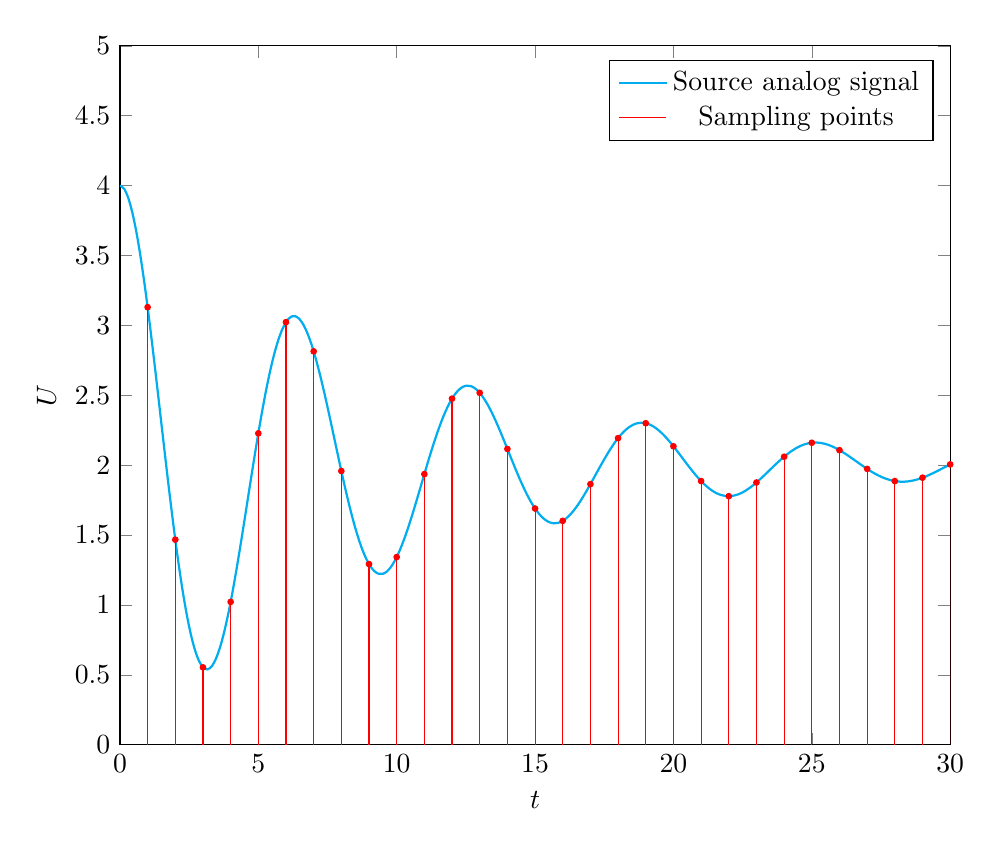
\begin{tikzpicture}
      [
        declare function={
          f(\x)=2 + exp(-\x/10)*( cos(deg(\x)) + sin(deg(\x))/10 ) * 2;
        }
      ]

      \begin{axis}[
          width = \textwidth,
	        xmin = 0, xmax = 30,
	        ymin = 0, ymax = 5.0,
          xlabel={$t$},
          ylabel={$U$}
        ]

	      \addplot[
		      domain = 0:30,
		      samples = 200,
		      smooth,
		      thick,
		      cyan
	      ] {
          2 + exp(-x/10)*( cos(deg(x)) + sin(deg(x))/10 ) * 2
        };

        \foreach \x [evaluate={\y=f(\x)}] in {1, 2, ..., 30} {
          \addplot[red]
          coordinates {
            (\x, 0) (\x, \y)
          };
          \addplot[red, mark = *, mark size=1.0pt]
          coordinates { (\x, \y) };
        };

        \legend{
	        Source analog signal,
          Sampling points
        }
	    \end{axis};
    \end{tikzpicture}
    \caption{Sampling.}
    \label{fig:adc-sampling-00}
  \end{figure}

  The frequency of those intervals is called \emph{sampling rate}.

    \begin{figure}[h]
    \centering
    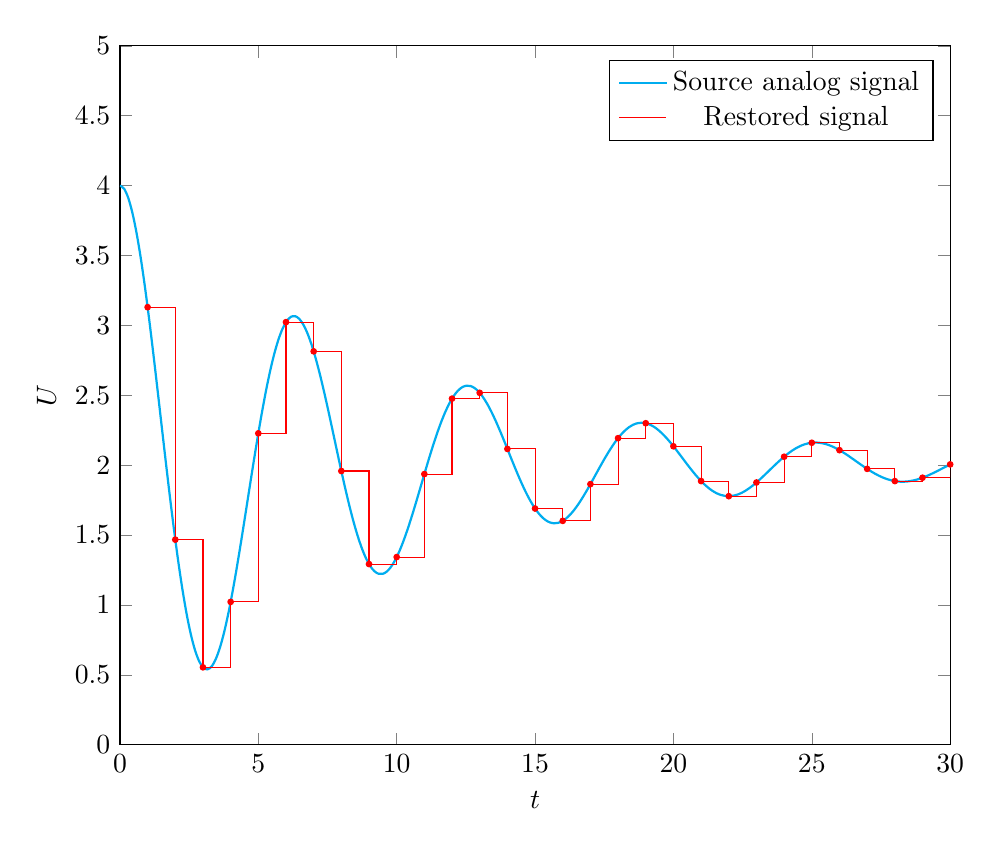
\begin{tikzpicture}
      [
        declare function={
          f(\x)=2 + exp(-\x/10)*( cos(deg(\x)) + sin(deg(\x))/10 ) * 2;
        }
      ]

      \begin{axis}[
          width = \textwidth,
	        xmin = 0, xmax = 30,
	        ymin = 0, ymax = 5.0,
          xlabel={$t$},
          ylabel={$U$},
        ]

	      \addplot[
		      domain = 0:30,
		      samples = 200,
		      smooth,
		      thick,
		      cyan
	      ] {
          2 + exp(-x/10)*( cos(deg(x)) + sin(deg(x))/10 ) * 2
        };

        \foreach \x [evaluate={\y=f(\x); \xnext=\x + 1; \ynext=f(\x + 1)}] in {1, 2, ..., 30} {
          \addplot[red]
          coordinates {
            (\x, \y) (\xnext, \y) (\xnext, \ynext)
          };
          \addplot[red, mark = *, mark size=1.0pt]
          coordinates { (\x, \y) };
        };

        \legend{
	        Source analog signal,
          Restored signal
        }
	    \end{axis}
    \end{tikzpicture}
    \caption{Rebuilding the source signal with recorded points.}
    \label{fig:adc-sampling-01}
  \end{figure}

    If we try to rebuild the source analog signal using the recorded points, we
    will get the graph similar to the one that is shown on
    fig. \ref{fig:adc-sampling-01}.  As we can see, some data got lost due to
    low sampling frequency -- that's why some parts of the graph were ``cut
    away.''

\item \textbf{Quantization.}  Acquired values are replaced with the closest
  values from the set of possible values -- \emph{quantization levels}.
  \index{Electronics!ADC!Quantization}

    \begin{figure}[h]
    \centering
    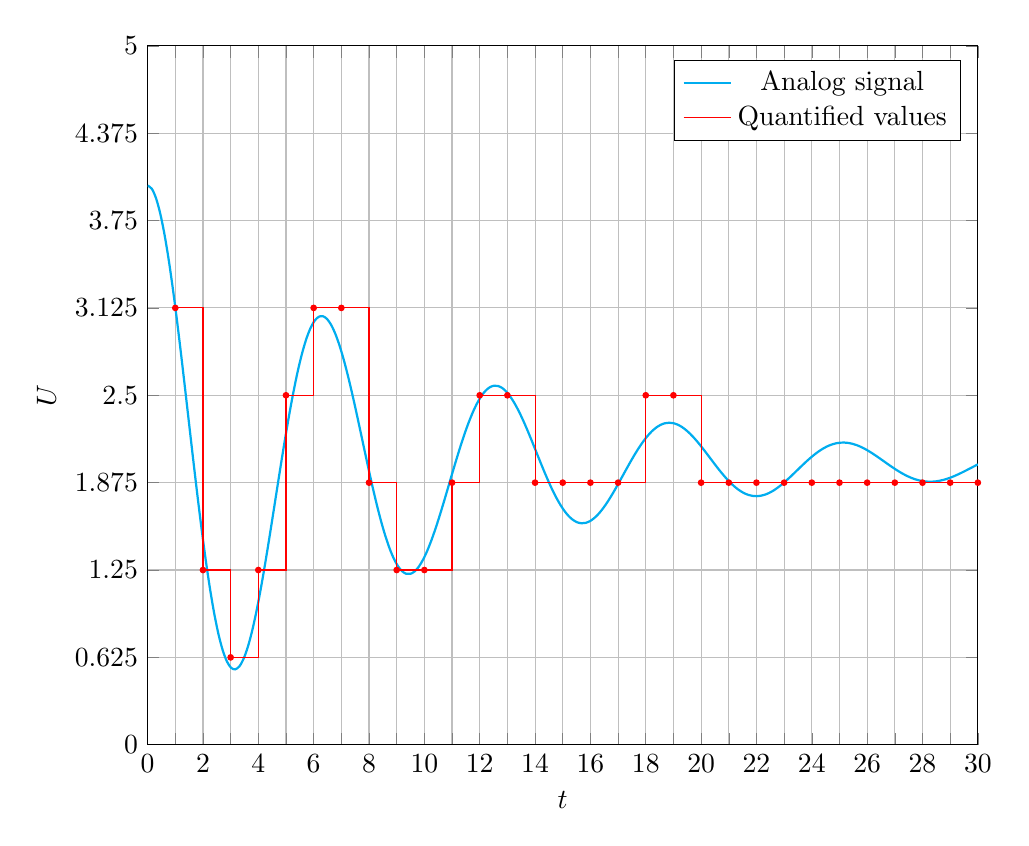
\begin{tikzpicture}
      [
        declare function={
          step=0.625;
          f(\x)=2 + exp(-\x/10)*( cos(deg(\x)) + sin(deg(\x))/10 ) * 2;
          q(\x)=mod(f(\x), step) == 0 ? f(\x) : ((int(round(f(\x) / step)) + 0) * step);
        }
      ]

      \begin{axis}[
          width = \textwidth,
	        xmin = 0, xmax = 30,
	        ymin = 0, ymax = 5.0,
          xlabel={$t$},
          ylabel={$U$},
          grid=both,
          grid style={line width=.2pt, draw=gray!10},
          major grid style={line width=.4pt,draw=gray!50},
          xtick distance = 1,
	        ytick distance = step,
          xtick = {0, 1, ..., 30},
          xticklabels={0,,2,,4,,6,,8,,10,,12,,14,,16,,18,,20,,22,,24,,26,,28,,30},
          /pgf/number format/precision=5
        ]

	      \addplot[
		      domain = 0:30,
		      samples = 200,
		      smooth,
		      thick,
		      cyan
	      ] {
          2 + exp(-x/10)*( cos(deg(x)) + sin(deg(x))/10 ) * 2
        };

        \foreach \x [evaluate={\y=q(\x); \xnext=\x + 1; \ynext=q(\x + 1)}] in {1, 2, ..., 30} {
          \addplot[red]
          coordinates {
            (\x, \y) (\xnext, \y) (\xnext, \ynext)
          };
          \addplot[red, mark = *, mark size=1.0pt]
          coordinates { (\x, \y) };
        };

        \legend{
	        Analog signal,
          Quantified values
        }
	    \end{axis}
    \end{tikzpicture}
    \caption{Quantization.}
    \label{fig:adc-quantization}
  \end{figure}

    The visual representation of the quantization process is shown on the
    fig. \ref{fig:adc-quantization}.  As we can see from the figure, in the
    quantified values we put points strictly on the cross-sections of the grid.
    The more horizontal lines in the grid, the closer we can set the value on
    the $y$ axis to the original value.

\item \textbf{Encoding.}  Binary codes are assigned to the resulting values (see
  \ref{fig:coding}.)
  \index{Electronics!ADC!Encoding}

  \begin{figure}[h]
    \centering
    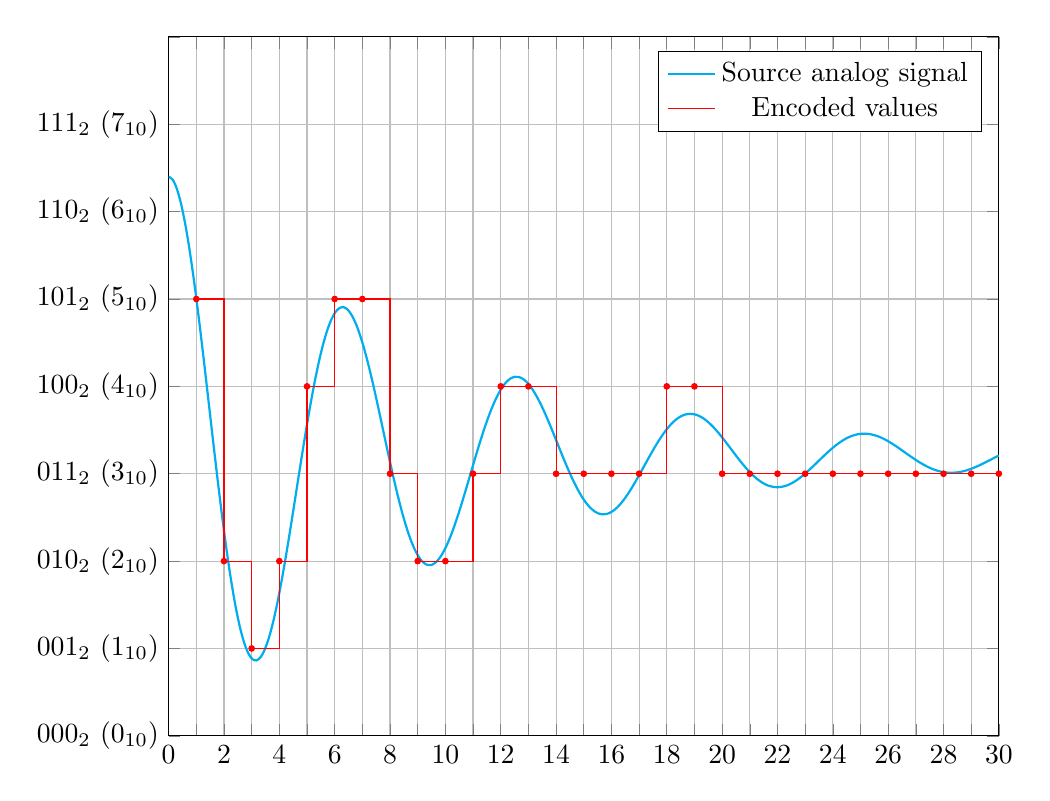
\begin{tikzpicture}
      [
        declare function={
          step=0.625;
          f(\x)=2 + exp(-\x/10)*( cos(deg(\x)) + sin(deg(\x))/10 ) * 2;
          q(\x)=mod(f(\x), step) == 0 ? f(\x) : ((int(round(f(\x) / step)) + 0) * step);
        }
      ]

      \begin{axis}[
          width = \textwidth,
	        xmin = 0, xmax = 30,
	        ymin = 0, ymax = 5.0,
          grid=both,
          grid style={line width=.2pt, draw=gray!10},
          major grid style={line width=.4pt,draw=gray!50},
          xtick distance = 1,
	        ytick distance = step,
          xtick = {0, 1, ..., 30},
          xticklabels={0,,2,,4,,6,,8,,10,,12,,14,,16,,18,,20,,22,,24,,26,,28,,30},
          /pgf/number format/precision=5,
          yticklabels={
            $000_2$ ($0_{10}$),
            $000_2$ ($0_{10}$),
            $001_2$ ($1_{10}$),
            $010_2$ ($2_{10}$),
            $011_2$ ($3_{10}$),
            $100_2$ ($4_{10}$),
            $101_2$ ($5_{10}$),
            $110_2$ ($6_{10}$),
            $111_2$ ($7_{10}$),
          }
        ]

	      \addplot[
		      domain = 0:30,
		      samples = 200,
		      smooth,
		      thick,
		      cyan
	      ] {
          2 + exp(-x/10)*( cos(deg(x)) + sin(deg(x))/10 ) * 2
        };

        \foreach \x [evaluate={\y=q(\x); \xnext=\x + 1; \ynext=q(\x + 1)}] in {1, 2, ..., 30} {
          \addplot[red]
          coordinates {
            (\x, \y) (\xnext, \y) (\xnext, \ynext)
          };
          \addplot[red, mark = *, mark size=1.0pt]
          coordinates { (\x, \y) };
        };

        \legend{
	        Source analog signal,
          Encoded values
        }
	    \end{axis};
    \end{tikzpicture}
    \caption{Encoding an analog signal in the binary form.}
    \label{fig:adc-encoding}
  \end{figure}

  An example of the 3-bit encoding is shown on the the
  fig. \ref{fig:adc-encoding}.

  The higher the sampling rate and the more quantization levels are available,
  the more precise is the analog-to-digital conversion.

\end{enumerate}

One of the main characteristics of the ADC is the \emph{resolution}.  It sets
the range for values that the ADC can output.

\index{Programming!Binary numeral system}

Computers are operating on the binary numeral system -- that is, the minimum
information storage unit, which is called \emph{bit}, can hold only one of the
two values: one or zero.

With two of such cells (bits) we can already store 4 combinations of the ones
and zeroes: 00, 01, 10, 11.  If we take 3 bits they will provide us with 8
combinations.  It's easy to see the pattern here: adding one additional bit
doubles the number of combinations.

We can calculate the number of combinations even easier: we don't have to put
ones and zeroes in imaginary ``cells'' and count them.  We can use the following
formula instead:

\begin{equation}
  \mbox{Number of combinations} = 2^{\mbox{n}}
\end{equation}

Where \texttt{n} is the number of available bits for storing some value.

For example, if we take 8 bits to store some data it will give us $2^8 = 256$
combinations of ones and zeroes.

Let's take a look on the graph on fig. \ref{fig:coding}: for encoding the values
we are using three bits -- thus, the ADC described by this graph, has the
resolution of 3 bits.  That is, the number of quantization levels is equal to
$2^3 = 8$.

But we should not forget that the counting in the computer world is usually
starts from zero, and the case when all the bits are set to zero, is the one of
the possible values.  Let's suppose we have 8 bits and we have set them to ones:
$11111111_2$.  If we convert this value into the decimal form we will get:

\begin{equation}
  11111111_2 = (2^7 * 1) + \mbox{...} + (2^2 * 1) + (2^1 * 1) + (2^0 * 1) = 255_{10}
\end{equation}

Thus we can see that the maximum positive value for 8 bits is equal to 255.

From that it follows that if we take 10 bits to store some information, we can
encode 1024 combinations of ones and zeroes, because $2^{10} = 1024$.  But the
maximum positive value will be equal to 1023.  Thus in Arduino the ADC has the
10-bits resolution.

Also there's a different system that is called \emph{digital-to-analog
converter} (DAC) which performs the inverse function of ADC -- that is, converts
a digital signal to an analog signal.

The use of ADCs and DACs is very widespread: it is used in audio/video cards, in
displays, in various audio equipment, in measurement devices (such as
oscilloscopes) and in many more areas.

We will discuss the DAC in the chapter \ref{chapter:pwm} titles ``Pulse-width
modulation.''

\subsection{Operation of ADC using temperature measurement as an example}
\label{subsection:adc-temperature-example}

Suppose we have to measure the air temperature outside our window to plot a
graph afterwards.  For this task we have to organize a table in the following
format:

\begin{table}[h]
  \centering
  \begin{tabular}{p{3cm}|p{4cm}}
    Measurement time & Temperature \\
    \hline \hline
    06:00 & -5 \\
    \hline
    12:00 & -7 \\
    \hline
    18:00 & -8 \\
    \hline
    00:00 & -10 \\
    \hline
  \end{tabular}
  \caption{An example data about air temperature variation.}
  \label{table:adc-temperature-data-example-1}
\end{table}

The measurements are taken in uniform time intervals and for each measurement
the timestamp and the air temperature is written down.

How can we improve the quality of our data?  There are two main parameters that
we can adjust:

\begin{itemize}
\item We can increase the \emph{frequency of the measurements}: if we perform
  measurements more often, it will allow us to register the dynamics of changes
  more precise.
\item We can increase the \emph{accuracy of measurements}: if we perform more
  accurate measurements, it will allow us to register smaller changes in the
  values.
\end{itemize}

An example of more frequent measurements (once in 3 hours) is shown in table
\ref{table:adc-temperature-data-example-2}.

\begin{table}[h]
  \centering
  \begin{tabular}{p{3cm}|p{4cm}}
    Measurement time & Temperature \\
    \hline \hline
    06:00 & -5 \\
    \hline
    09:00 & -4 \\
    \hline
    12:00 & -7 \\
    \hline
    15:00 & -8 \\
    \hline
    18:00 & -8 \\
    \hline
    21:00 & -9 \\
    \hline
    00:00 & -10 \\
    \hline
  \end{tabular}
  \caption{An example data about air temperature variation with more frequent
    measurements.}
  \label{table:adc-temperature-data-example-2}
\end{table}

If we also increase the accuracy of measurements, we will get the table similar
to подобную \ref{table:adc-temperature-data-example-3}.

\begin{table}[h]
  \centering
  \begin{tabular}{p{3cm}|p{4cm}}
    Measurement time & Temperature \\
    \hline \hline
    06:00 & -5.2 \\
    \hline
    09:00 & -4.1 \\
    \hline
    12:00 & -7.2 \\
    \hline
    15:00 & -8.5 \\
    \hline
    18:00 & -8.9 \\
    \hline
    21:00 & -9.0 \\
    \hline
    00:00 & -10.7 \\
    \hline
  \end{tabular}
  \caption{An example data about air temperature variation with more frequent
    and more accurate measurements.}
  \label{table:adc-temperature-data-example-3}
\end{table}

In case of ADC, the increase in the frequency of measurements is called the
increase in sampling rate.  In this regard, the increase in recording accuracy
is called the increase in resolution of the converter.

In case of ADC a computer measures the voltage on the analog input (for example,
from a temperature sensor.)  After that the analog-to-digital conversion takes
place where each voltage value is assigned some digital value from the available
range, set by the converter resolution.

As the result, for example, in case of -5.2 degrees Celsius on a thermometer, a
computer may read it as the value of 1.3 Volts.  Further, a digital value of
$01110101_2$ ($117_{10}$) is assigned to this value (see
\ref{table:adc-temperature-data-example-4}.

\begin{table}[h]
  \centering
  \begin{tabular}{p{3cm}|p{4cm}|p{4cm}}
    Measurement time & Temperature & The ADC output value \\
    \hline \hline
    06:00 & -5.2  & 117 \\
    \hline
    09:00 & -4.1  & 121 \\
    \hline
    12:00 & -7.2  & 109 \\
    \hline
    15:00 & -8.5  & 104 \\
    \hline
    18:00 & -8.9  & 103 \\
    \hline
    21:00 & -9.0  & 102 \\
    \hline
    00:00 & -10.7 & 95 \\
    \hline
  \end{tabular}
  \caption{An example of data with binary encoding.}
  \label{table:adc-temperature-data-example-4}
\end{table}

\subsection{Using ADC to record a sound}
\index{Electronics!ADC!Sound recording}

Sound recording is a good example that we can use to learn some practical
application of ADC.  A sound wave receiver is usually a microphone that have a
construction similar to a speaker, but has inverse functionality to it:

\begin{itemize}
\item In a speaker, changing electric current in a coil creates a magnetic field
  that interacts with a permanent magnet which in turn makes a speaker membrane
  to vibrate -- and that creates sound waves.
\item In a microphone, sound waves make a membrane vibrate.  The membrane is
  attached to a permanent magnet, that is enclosed inside a coil.  When the
  permanent magnet moves inside a coil, it creates the electric current that can
  be measured.
\end{itemize}

Sound recording is a regular measurement of voltage values on the microphone
coil.  Each measurement is attached to the timestamp where this measurement was
performed.

As in the case with the temperature measurement in the section
\ref{subsection:adc-temperature-example}, the quality of sound recording depends
on the frequency of measurements (\emph{sampling rate}) and the ADC resolution.

Some examples of the standard sampling rates for audio are shown in the table
\ref{table:adc-sound-sampling-rate-1}.  Sampling rate directly affects the
maximum frequency of the sound that can be recorded.  Theoretically the maximum
frequency that can be recorded is the half of the sampling rate (so called the
Nyquist frequency.)  But in reality this limit is slightly lower so the maximum
sound frequency for the sampling rate of 44100Hz is a little bit higher than
20000Hz, but lesser than 22050Hz. \cite{audacityteam:sample-rates}

\begin{table}[h]
  \centering
  \begin{tabular}{p{2cm}|p{9cm}}
    Sampling rate & Applications \\
    \hline \hline

    8000 Hz & Old telephone line, walkie-talkie.  Not good for the most of the
    tasks, but can be useful for some sound effects and to recording the
    infra-sound (sound frequencies that are lower than a human ear can hear.) \\

    \hline

    11025 Hz & This sampling rate is used to record some low-quality sound. \\

    \hline

    22050 Hz & Half of the sampling rate that is used on CDs.  Suitable for
    digitization of old audio recordings from the 20th century.  Also used for
    recording human speech where the quality of the sound is not important, but
    the clearness of the speech have to be maintained. \\

    \hline

    32000 Hz & Suitable for the digitizing of tape recordings and for recording
    human speech. \\

    \hline

    44100 Hz & The standard quality of audio recordings in CDs.  It allows us to
    record sound frequencies up to 20KHz, which is considered the limit of human
    hearing range for the most people. \\

    \hline

    48000 Hz & This standard is used for audio encoding on DVDs. \\

    \hline

    96000 Hz & Audio recordings on DVDs and Blu-ray disks. \\

    \hline

    192000 Hz & Used on DVDs and Blu-ray disks as well.  This quality is often
    used in the professional audio recording equipment. \\

    \hline

  \end{tabular}
  \caption{Some standard sampling rates for audio recording.}
  \label{table:adc-sound-sampling-rate-1}
\end{table}

Bit depth (also known as \emph{resolution}) determines how many bits will be
used for encoding of each measured value.  Thus, this parameter sets the
accuracy of the recorded signal.  The more bit depth we have, the more different
discrete values we can use to store a value.  \cite{audacityteam:bit-depth}

Some examples of the common bit depths for sound recording are shown in the
table \ref{table:adc-sound-bit-depth-1}.

\begin{table}[h]
  \centering
  \begin{tabular}{p{2cm}|p{9cm}}
    Bit depth & Description \\
    \hline \hline

    8 bits & Low-quality sound, comparable to the sound quality of the old
    analog telephone lines. \\

    \hline

    16 bits & CD-audio quality. \\

    \hline

    24 bits & This bit depths is used for the sound recording for the afterward
    processing.  More bits are taken so even after all the processing the
    quality will be good enough for producing the 16-bit CD-audio quality. \\

    \hline

    32 bits & This bit depth is used for maintaining the highest standards of
    sound recording quality.  It is used for the situations where elaborate
    sound processing is expected before exporting to other formats. \\

    \hline

  \end{tabular}
  \caption{Some common bit depths used in sound recording.}
  \label{table:adc-sound-bit-depth-1}
\end{table}

Here we can mention 8-bit music.  Its name represents the 8-bit depth resolution
of the ADC and DAC of the sound chips of those old game consoles for which this
kind of music was made.  The main theme from the game ``Super Mario Bros.'' that
was written for the Nintendo Entertainment System (NES) in the year 1985 is a
good example of such music.  This low bit depth is the explanation for the
characteristic sound of the old game consoles.

\subsection{ADC in the digital photography and video-recording}
\index{Electronics!ADC!Image digitization}

\newglossaryentry{FPS}{name=FPS, description={Frames Per Second.}}

Another example of \gls{ADC} application is the digital photography.  In a
digital camera a lens focuses light onto a special matrix made from miniature
solar cells (``pixels''), where each pixel captures beams of light and converts
them into electric signals. \cite{expertphotography}

In the black-and-white camera each pixel represents a light intensity detector.
The more sensible the detector, the more levels of the signals we can get on the
output.  In a color digital camera, as each pixel is sensible only to limited
range of light spectrum, to catch images we need three kinds of pixels: red,
green and blue.  Those pixels are organized in the pattern which is called
``Bayer filter'' where three kinds of pixels are grouped together into bigger
``cells'' from the four pixels: blue, green, green, red.

For image digitization an ADC converts the input electric signals from the
light-sensitive matrix into digital values, according to the resolution of the
converter.  For example, the 8-bit resolution will give us 256 levels of light
intensity of each parts of the spectrum.

The acquired values then stored in the form of matrix into a file that is called
\emph{an image}.  If we take a black-and-white camera with the resolution of
16x16 pixels it will give us an image of $16 * 16 = 256$ pixels in size.  If the
ADC has the resolution of 8 bits then the amount of image data can be calculated using the following equation:

\begin{equation}
  \mbox{Amount of data} = 16 * 16 * 8 = 2048 \mbox{bits} = 256 \mbox{bytes}
  \label{equation:adc-image-0}
\end{equation}

For colorful images the amount of stored data is bigger, because we need to
store three color components: red, green and blue (in the RGB format.)  If we
also take the 8-bits ADC then each pixel we need to store $8 * 3 = 24$ bits of
information.  Let's take another look at the example with 16x16 pixels camera
and substitute new values to the equation:

\begin{equation}
  \mbox{Amount of data} = 16 * 16 * 24 = 6144 \mbox{bits} = 768 \mbox{bytes}
  \label{equation:adc-image-1}
\end{equation}

Here we have to note that we have yet to mention the sampling rate in the
context of digital photography.  It's no wonder as the image capturing is a
single operation that produces one image.  The \emph{frame rate} parameter
(measured in frames per second, or \gls{FPS}) that controls the speed of image
digitization, appears only when a sequential capturing of several images is
performed -- which is usually used for capturing a \emph{video}.

The more is frame rate in video capturing, the more information we can capture
and thus the more precisely we can track fast objects movement that are in the
focus of the camera.

The standard frame rate is 24 \gls{FPS} that allows us to get sufficiently
smooth movements in the video.  Another popular frame rate is 30 FPS and 60 FPS.
For the high-speed video shooting that allows us to get the ``slow motion''
effect, frame rates such as 120 FPS or more are used.

If we assume that a colorful video camera has the resolution of 16x16 pixels and
we use it to capture 10 seconds of video with 24 FPS, then the total number of
frames in the video will be:

\begin{equation}
  \mbox{Frames} = 24 * 10 = 240 \mbox{frames}
\end{equation}

The size of one frame will be 768 bytes as is shown in the equation
\ref{equation:adc-image-1}.

Then the total size of output video data will be:

\begin{align}
  \mbox{Video-file size} & = 768 \mbox{bytes per frame} * 240 \mbox{frames} \\
  & = 184320 \mbox{bytes} \\
  & = 180 \mbox{Kb}
  \label{equation:adc-image-2}
\end{align}

Now it is important to note that currently we consider only storing the ``raw''
data (that is, data in the original form), without any compression.  Compression
of digitized data is a separate topic and currently we will not discuss it the
book in details.

For the completeness sake we can say that there are two kinds of compression:
\begin{itemize}
\item \textbf{Lossless compression} -- the source data is compressed in such a
  way that no parts of data is lost so after the de-compression all the original
  data will be restored.  The compression rate usually is not very high.
\item \textbf{Lossy compression} -- the source data is processed with specialized
  algorithms aimed to remove ``extra'' (or ``not very important'') information
  (from the point of human perception), thus allowing us to achieve way better
  compression ratio that in the case of lossless compression algorithms.  But we
  won't be able to fully restore the original data from the compressed data.  If
  we take the compressed data and process it with the same compression algorithm
  that is used to compress it in the first place we will make the quality of
  data even worse.
\end{itemize}

For example, one of the lossless compression formats for images is ``Portable
Network Graphics'' format (or PNG.)  On contrary, we can take the JPG format as
an example of lossy compression.

\end{document}

